\documentclass[a4paper,11pt]{article}

%%%%%%%%%%%%%%%%%%%%%%%%%%%%%%%%%%%%%%%%%%%%%%%%%%%%%%%%%%%%%%%%%%%%%%%%
% Paquetes utilizados
%%%%%%%%%%%%%%%%%%%%%%%%%%%%%%%%%%%%%%%%%%%%%%%%%%%%%%%%%%%%%%%%%%%%%%%%

% Gráficos complejos
\usepackage{graphicx}
\usepackage{caption}
\usepackage{subcaption}
\usepackage{placeins}

% Soporte para el lenguaje español
\usepackage{textcomp}
\usepackage[utf8]{inputenc}
\usepackage[T1]{fontenc}
\DeclareUnicodeCharacter{B0}{\textdegree}
\usepackage[spanish]{babel}

% Código fuente embebido
\usepackage{listings}

% PDFs embebidos para el apéndice
\usepackage{pdfpages}

% Matemáticos
\usepackage{amssymb,amsmath}

% Tablas complejas
\usepackage{multirow}

% Formato de párrafo
\setlength{\parskip}{1ex plus 0.5ex minus 0.2ex}

%%%%%%%%%%%%%%%%%%%%%%%%%%%%%%%%%%%%%%%%%%%%%%%%%%%%%%%%%%%%%%%%%%%%%%%%
% Título
%%%%%%%%%%%%%%%%%%%%%%%%%%%%%%%%%%%%%%%%%%%%%%%%%%%%%%%%%%%%%%%%%%%%%%%%

% Título principal del documento.
\title{\textbf{Trabajo Práctico 1: Conjunto de Instrucciones MIPS}}

% Información sobre los autores.
\author{\\
  Guido Laghi, \textit{P. 82.449}                                  \\
  \texttt{guido321@gmail.com}                                      \\ [2.5ex]
  Sebastián L. Pérez, \textit{P. 84.379}                           \\
  \texttt{sebastian.leo.perez@gmail.com}                           \\ [2.5ex]
  Sergio Matías Piano, \textit{P. 85.191}                          \\
  \texttt{smpiano@gmail.com}                                       \\ [2.5ex]
                                                                   \\
  \normalsize{1er. Cuatrimestre de 2013}                           \\
  \normalsize{66.20 Organización de Computadoras}                  \\
  \normalsize{Facultad de Ingeniería, Universidad de Buenos Aires} \\
}
\date{}

%%%%%%%%%%%%%%%%%%%%%%%%%%%%%%%%%%%%%%%%%%%%%%%%%%%%%%%%%%%%%%%%%%%%%%%%
% Documento
%%%%%%%%%%%%%%%%%%%%%%%%%%%%%%%%%%%%%%%%%%%%%%%%%%%%%%%%%%%%%%%%%%%%%%%%

\begin{document}

% ----------------------------------------------------------------------
% Top matter
% ----------------------------------------------------------------------
\thispagestyle{empty}
\maketitle

\begin{abstract}

  Este informe sumariza el desarrollo del trabajo práctico 1 de la materia
  Organización de Computadoras (66.20) dictada en el primer cuatrimestre de
  2013 en la Facultad de Ingeniería de la Universidad de Buenos Aires. El mismo
  consiste enla construcción de un sistema minimalista de ordenamiento de
  archivos y el análisis de performance y perfilado del mismo, con foco en la
  generación de un entorno de infraestructura básica para soportar el
  desarrollo de estas tareas que será reutilizado en futuros trabajos
  prácticos.

\end{abstract}

\clearpage

% ----------------------------------------------------------------------
% Tabla de contenidos
% ----------------------------------------------------------------------
\tableofcontents
\clearpage


% ----------------------------------------------------------------------
% Desarrollo
% ----------------------------------------------------------------------
\part{Desarrollo}

\section{Introducción}

El proceso de compilación de un programa codificado en C consiste en un
pipeline que genera finalmente código objeto para una arquitectura objetivo.
Este pipeline analiza y traduce el código a diferentes representaciones de los
algoritmos contenidos en él, de manera de terminar generando código objeto que
finalmente se linkea en un ejecutable válido para la arquitectura.

Debido a que el lenguaje C es un lenguaje de alto nivel, varios de los
conceptos propios de este lenguaje deben ser mapeados a diferentes estrategias
que pueden ser ejecutadas en el código objeto, que no es más que el conjunto de
instrucciones que la arquitectura objetivo provee. Estos mapeos muchas veces
pueden implementarse de diferentes maneras, cada una con sus ventajas y
desventajas, y si bien el compilador realiza una muy buena tarea en determinar
la mejor manera en la que traducir estos conceptos en instrucciones de bajo
nivel, los algoritmos utilizados no garantizan que la traducción sea de manera
de generar el código objeto más eficiente y compacto que se podría tener.

La alternativa que se propone explorar en el presente trabajo es la
implementación directa en assembly de las rutinas del sistema que se está
construyendo. Esta alternativa tiene una característica fundamental: al tener
acceso al conjunto de instrucciones que ejecuta la arquitectura potencialmente
se puede desarrollar una solución óptima, minimizando el acceso a memoria, la
cantidad de instrucciones a ejecutar, etc.

Por otro lado, la implementación en assembly de un sistema no trivial es una
tarea complicada. La dificultad principal radica en que es tarea del
programador implementar y controlar muchos de los mecanismos de bajo nivel que
constituyen el \textit{cómo} de la solución, en vez de concentrarse en el
\textit{qué}. Algunos ejemplos son el manejo del stack, la implementación de
convenciones de llamadas de subrutinas, el uso de registros compartidos, entre
otros.

\section{Implementación}

El sistema que resuelve el problema planteado en el enunciado (disponible en el
anexo \ref{sec:enunciado}) fue implementado mayoritariamente en C, y parte en 
lenguaje MIPS como lo indicaba el enunciuado. La diferencia fundamental radica 
en la implementación de las rutinas de ordenamiento a través del algoritmo 
\textit{shellsort} directamente en assembly. El código fuente de
la solución está disponible en el anexo \ref{sec:source}; por cuestiones de
espacio y prolijidad sólo se incluyen los archivos relacionados con la
implementación en assembly de la solución desarrollada.

Cabe destacar que la solución en assembly definitivamente no es la solución
óptima. Existen algunas mejoras posibles para disminuir la cantidad de
instrucciones a ejecutar o los accesos a memoria: por ejemplo, se podrían
reordenar las instrucciones de algunos de los bloques de los procedimientos
implementados para eliminar algunas de las instrucciones de salto
incondicional, o se podrían utilizar de mejor manera los registros salvados
(s0-s8) para eliminar la necesidad de restaurar desde el stack algunos de los
registros en uso (particularmente a0, a1 y a2 en la implementación de
\textit{shell\_sort\_s}). Sin embargo, dado que la solución que se presenta
contiene el \(40\%\) de las instrucciones del equivalente implementado en C
compilado sin optimizaciones, a los efectos del trabajo práctico consideramos
suficientemente óptima la implementación propuesta.

A continuación enumeraremos algunas consideraciones de diseño tomadas al
implementar cada una de las funciones involucradas en el algoritmo de
ordenamiento.

\subsection{shell\_sort\_s}

Esta función implementa el ordenamiento de una tabla de strings a través de
\textit{shellsort}. El método de ordenamiento fue implementado en su forma más
sencilla a través de un algoritmo recursivo. El stack frame típico de la
función se describe a continuación en la figura \ref{fig:stackshell}.

\begin{figure}[h!]
  \centering
  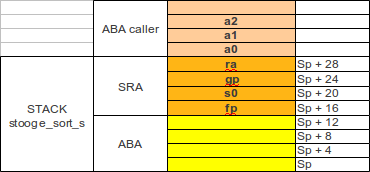
\includegraphics[width=\textwidth]{docs/stack_stooge_sort_s.png}
  \caption{Diagrama de stack para la función shell\_sort\_s} \label{fig:stackshell}
\end{figure}

\FloatBarrier

Se reservan 16 bytes para el área de SRA: 4 bytes para salvar el registro ra en
llamadas a otras funciones, 4 bytes para salvar el registro gp, 4 bytes para
preservar el registro s0 utilizado en varios de los cálculos de la función y
finalmente 4 bytes para el registro fp.

Por otro lado, dado que las funciones invocadas desde esta no poseen nunca más
de tres argumentos, se reservan \(4 x 4\) bytes en concepto de ABA para ser
utilizados por las funciones llamadas.

Esta función invoca tanto a \textit{compare\_s} como a \textit{swap\_s}, además
de las invocaciones recursivas mencionadas anteriormente.

\subsection{compare\_s}

Esta función compara byte a byte dos cadenas de caracteres terminadas en 0
(siguiendo la convención de C). Devuelve un número negativo si la primer cadena
es anterior a la segunda, 0 si son iguales o un número positivo si la primer
cadena es posterior a la segunda. El stack frame típico de la función se
describe a continuación en la figura \ref{fig:stackcompare}.

\begin{figure}[h!]
  \centering
  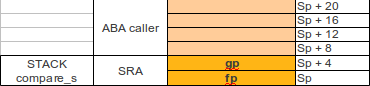
\includegraphics[width=\textwidth]{docs/stack_compare_s.png}
  \caption{Diagrama de stack para la función compare\_s} \label{fig:stackcompare}
\end{figure}

\FloatBarrier

Esta función fue implementada como leaf, sin invocar otras funciones
auxiliares. Se reservan 8 bytes para salvar gp y fp. No es necesario reservar
espacio adicional para ABA.

\subsection{swap\_s}

Esta función intercambia las cadenas ubicadas en dos posiciones dadas dentro de
una tabla de cadenas. El stack frame típico de la función se describe a
continuación en la figura \ref{fig:stackswap}.

\begin{figure}[h!]
  \centering
  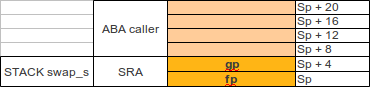
\includegraphics[width=\textwidth]{docs/stack_swap_s.png}
  \caption{Diagrama de stack para la función swap\_s} \label{fig:stackswap}
\end{figure}

\FloatBarrier

Nuevamente, esta función leaf no requiere reservar espacio adicional para ABA.
El stack es idéntico al de la función compare\_s, con 8 bytes para salvar gp y
fp únicamente.

\section{Compilación}

Se instrumentó un \textit{makefile} para ejecutar las instrucciones adecuadas
de compilación para los distintos escenarios requeridos. La
tarea \textit{make} compila individualmente cada uno de los archivos fuente de
extensión \textit{c} y \textit{S} a través del ejecutable \textit{gcc}.
Los comandos utilizados para compilar cada uno de estos archivos fuente son los
siguientes:

\begin{lstlisting}
gcc -c -o build/obj/buffer.o source/buffer.c -I./source -Wall
gcc -c -o build/obj/data.o source/data.c -I./source -Wall
gcc -c -o build/obj/clargs.o source/clargs.c -I./source -Wall
gcc -c -o build/obj/cltext.o source/cltext.c -I./source -Wall
gcc -c -o build/obj/tp1.o source/tp1.c -I./source -Wall
gcc -c -o build/obj/stoogec.o source/shellsort.c -I./source -Wall
gcc -c -o build/obj/stoogeasm.o source/shellsort.S -I./source -WalL
\end{lstlisting}

De este listado, cada una de las invocaciones obedece a la siguiente estructura
de argumentos:

\begin{description}

  \item[-c] Compila o ensambla el código fuente pero no corre el linker.  Por
    lo tanto la salida corresponde a un archivo objeto por cada archivo fuente.

  \item[-o] Especifica cual será el archivo de salida sea éste un archivo
    objeto, ejecutable, ensamblado o código preprocesado de C.

  \item[-Wall] Activa todos los mensajes de warning.

  \item[-I] Agrega el directorio especificado a la lista de directorios
    buscados para los archivos header

\end{description}

El resultado de la ejecución de estos comandos es que se generan archivos
objeto para cada fuente, listos para ser linkeados, en el directorio
\textit{build/obj}. Para realizar este último paso, se invoca nuevamente a
\textit{gcc} con un último comando:

\begin{lstlisting}
gcc -o build/tp0 \
  build/obj/buffer.o build/obj/data.o \
  build/obj/clargs.o build/obj/cltext.o \
  build/obj/tp1.o build/obj/stoogec.o build/obj/stoogeasm.o
\end{lstlisting}

El comando linkea todos los archivos objeto en un ejecutable final,
\textit{build/tp1}.

\section{Análisis de tiempos de ejecución}

En las siguientes secciones detallaremos el proceso de análisis de tiempo de
ejecución realizado para los diferentes casos contemplados.

\subsection{Análisis previo}\label{sec:tiempos}

El análisis de tiempos de ejecución se focalizará en comparar la performance de
la implementación en assembly descripta anteriormente contra diferentes
versiones de esencialmente el mismo sistema.

Primero se comparará el desempeño de los algoritmos escritos en C. utilizando todas las optimizaciones disponibles por el
compilador. Se espera nuevamente encontrar algunas mejoras, aunque pequeñas,
con respecto a lo que puede entregar el compilador.

Luego se comparará el algoritmo escrito en C contra el mismo en lenguaje ensabmblador.
Por un lado, al compilar esta solución sin ninguna optimización del compilador 
se espera obtener ganancias de performance apreciables, debidas mayormente al 
mejor manejo de los accesos a memoria logrados por el ejecutable desarrollado en assembly.

\subsection{Experimentos}

Se realizaron pruebas utilizando los archivos provistos por la cátedra sobre un entorno de ubuntu actual y sobre el emulador GXemul.
Obtuvimos los siguientes resultados:

Ubuntu:

**** bubblesort **** 
alice 0m 13.107s
beowulf 0m 20.749s
cyclopedia 3m 27.744s
elquijote 60m 32.782s


**** shellsort **** 
alice 0m 0.422s
beowulf 0m 0.537s
cyclopedia 0m 1.920s
elquijote 0m 5.675s

GXemul:

**** bubblesort **** 
alice 15m 17.180s
beowulf 27m 11.102s
cyclopedia [.infinito.]
elquijote [.infinito.]


**** shellsort **** 
alice 0m 7.281s
beowulf 0m 9.500s
cyclopedia 0m 29.234s
elquijote 2m 8.613s

\begin{table}[h!t]
\centering
\begin{tabular}{ | l | r | }
  \hline
  Ejecutable          & Tiempo de ejecución (s) \\ \hline
  Shellsort assembly & \(4.230\) \\
  Shellsort C O0     & \(9.960\) \\
  Shellesort C O3     & \(4.867\) \\
  Bubblesort C O0      & \(0.143\) \\
  Bubblesort C O3      & \(0.073\) \\
  \hline
\end{tabular}
\caption{Medición de tiempos de ejecución para cada experimento}
\label{tab:resultados}
\end{table}

\FloatBarrier

Se observaron todos los resultados esperados. Si bien hubo una mejoría
apreciable en el tiempo de ejecución de la implementación en assembly contra la
de C sin optimizaciones de compilador (más del 50\% de ganancia), la
compilación con todas las optimizaciones activadas se mantuvo relativamente
cerca de nuestra implementación particular.

Por otro lado, como era de esperarse, la implementación por \textit{quicksort}
fue muchísimo más performante que nuestra versión optimizada manualmente,
tomando menos del 10\% del tiempo de ejecución de nuestra versión incluso en la
versión compilada sin optimizaciones del compilador.

\section{Conclusiones}

La implementación en assembly del trabajo práctico, incluso cuando este se
trataba de un algoritmo relativamente simple y sencillo de desarrollar, fue
relativamente complicado. Como se explicó en secciones anteriores, gran parte
de la dificultad inherente en este desarrollo se encuentra en la necesidad de
implementar, administrar y controlar la infraestructura de los llamados a
funciones y otros artefactos básicos de integración. Por otro lado, el código
de ensamblador no provee muchas de las abstracciones básicas que se dan por
sentado en los lenguajes de alto nivel, como bloques condicionales y conversión
de tipos, lo que hizo que la implementación del algoritmo sea aún más
dificultoso: el \textit{qué} estábamos haciendo se mezclaba con el
\textit{cómo}. Por último, la ausencia de mecanismos de seguridad presentes en
lenguajes compilados, como la comprobación de tipos, prototipos funcionales y
declarativas en la asignación de nombres a variables incrementó la cantidad
de bugs con los que nos topamos, lo que dio a lugar a más trabajo de depuración
y testing.

El costo adicional de implementación fue claro: mientras que la versión en C
fue diseñada, implementada y testeada en 4 horas de trabajo de uno de los
integrantes del trabajo práctico, su equivalente en assembly nos llevó a dos
integrantes varios días de trabajo, particularmente en el testing y depuración
de errores. Si bien puede atribuirse esto a la falta de experiencia en
programación a bajo nivel, el resultado sigue siendo que el desarrollo es mucho
más costoso.

Teniendo en cuenta estos factores, entendemos que es imperativo el análisis de
costo-beneficio al decidirse por una implementación de este tipo. En nuestro
caso particular, la diferencia en tiempo de ejecución de nuestra solución
contra la producida por un compilador con todas las optimizaciones disponibles
habilitadas está dentro del 10\%. ¿Justifica el enorme costo adicional esa
ganancia?

Analizando el resto de los resultados concluimos que la versión implementada en
C con \textit{quicksort}, incluso cuando no se aplicaron optimizaciones de
compilador, era un orden de magnitud más eficiente que la versión implementada
en assembly. Esta versión fue desarrollada, depurada y testeada por un
integrante en el transcurso de un día, con un costo total de implementación
mucho menor a lo necesario para la versión assembly.

Como en todas las ingenierías, nuestro trabajo se basa en nuestra capacidad de
analizar alternativas y balancear costos y beneficios. En nuestro caso
particular, la implementación en assembly del sistema no era conveniente.
Realizando un análisis previo fácilmente podíamos concluir que para mejorar la
performance era mejor la alternativa de cambiar el algoritmo de ordenamiento
antes que invertir tiempo y esfuerzo en realizar la conversión.

Esta conclusión contradice la creencia generalizada de que la implementación
más eficiente se logra descartando las abstracciones de las que disponemos. No
siempre que se desarrolle una solución al más bajo nivel posible se llegará a
la solución más óptima. Y aún cuando sea la óptima, hay que evaluar si el costo
adicional incurrido justifica las ganancias obtenidas.

\clearpage

\part{Apéndice}
\appendix

\section{Enunciado original}\label{sec:enunciado}
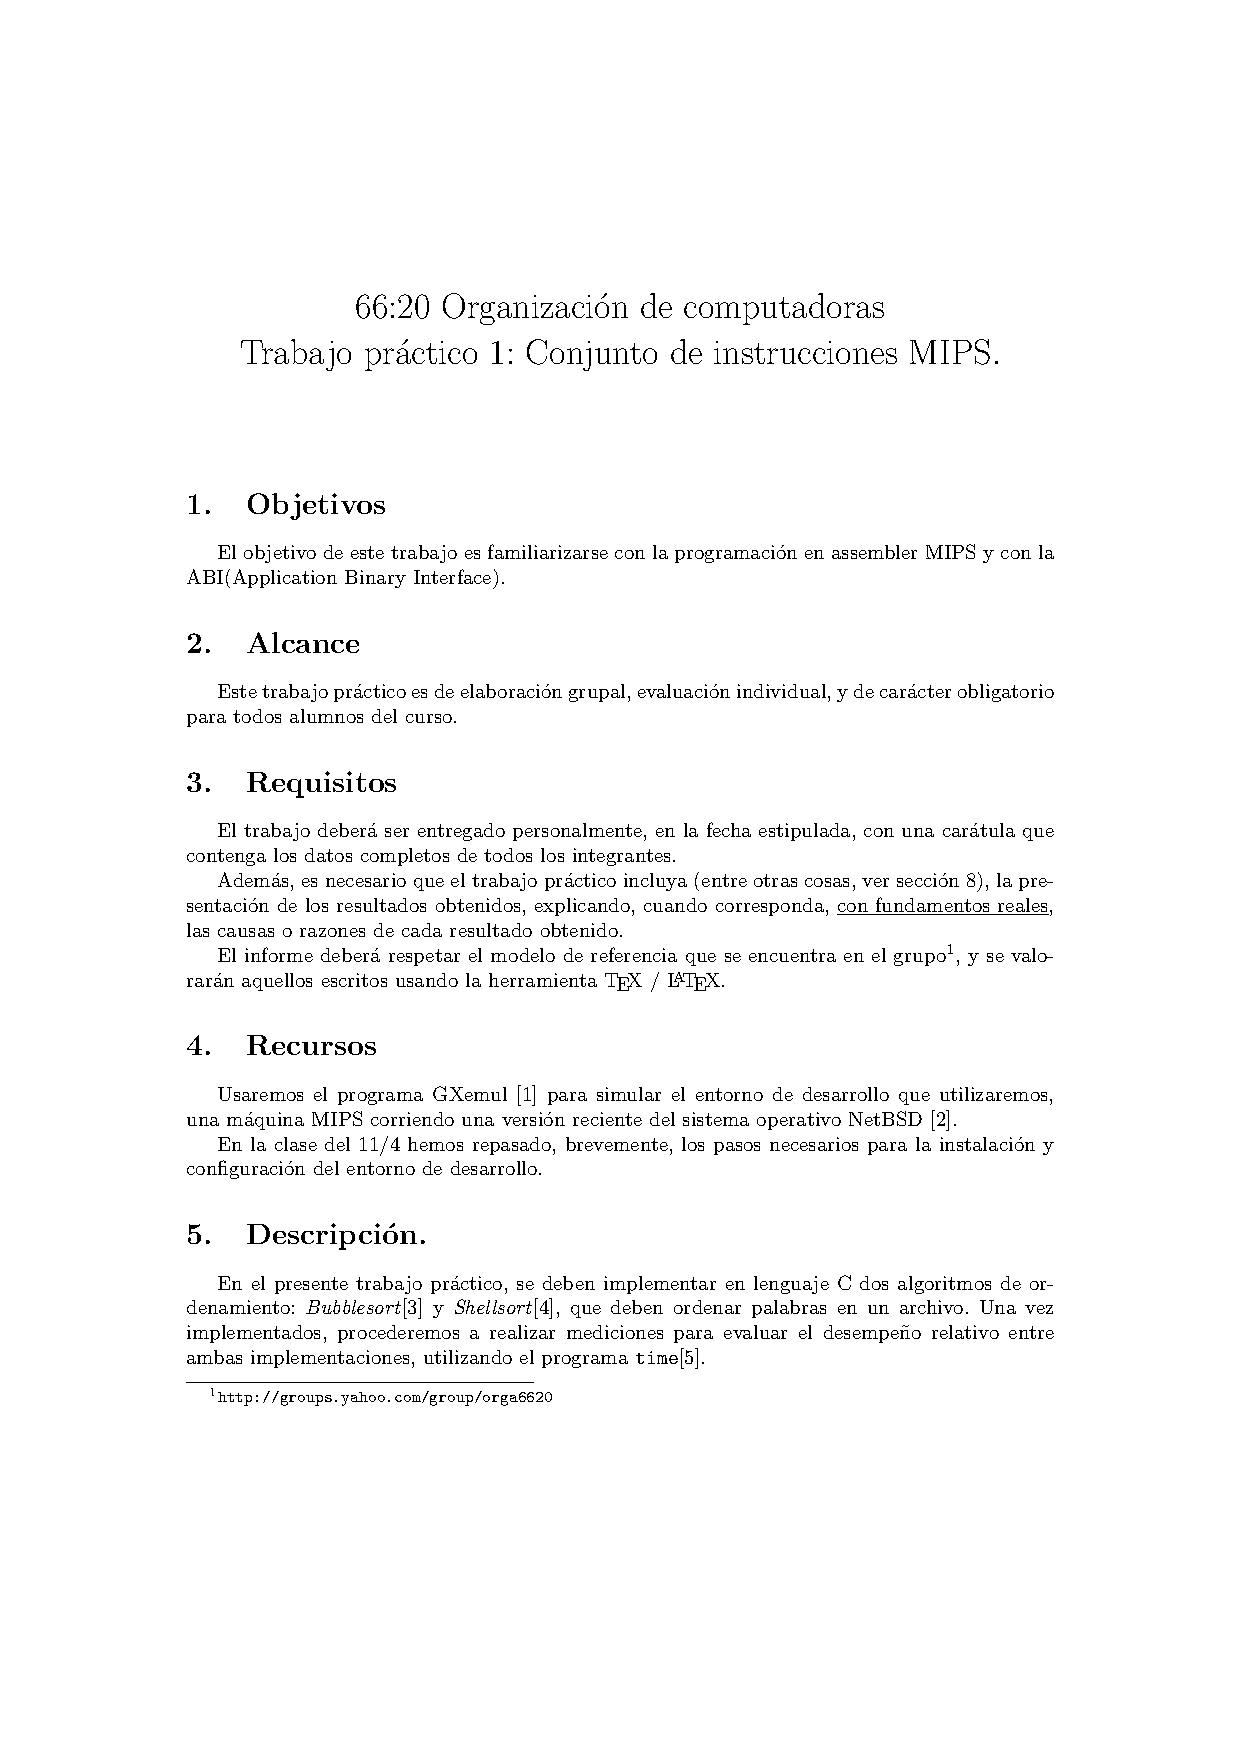
\includepdf[pages={-}]{docs/enunciado.pdf}

\clearpage
\section{README del material digital}\label{sec:readme}
\includepdf[pages={-}]{build/doc/README.pdf}

\clearpage
\section{Código fuente}\label{sec:source}
\clearpage
\definecolor{gray}{rgb}{0.5,0.5,0.5}
\lstset{
  title=\lstname,
  basicstyle=\footnotesize,
  showspaces=false,
  showstringspaces=false,
  breaklines=true,
  commentstyle=\color{gray},
  numbers=left,
  numberstyle=\tiny\color{gray},
  numbersep=5pt,
  frame=single
}

%\lstinputlisting{source/shellsort.h}
%\lstinputlisting{source/shellsort.S}

\end{document}
